% Options for packages loaded elsewhere
% Options for packages loaded elsewhere
\PassOptionsToPackage{unicode}{hyperref}
\PassOptionsToPackage{hyphens}{url}
\PassOptionsToPackage{dvipsnames,svgnames,x11names}{xcolor}
%
\documentclass[
  british,
  8.6pt,
  a4paper,
  twocolumn]{article}
\usepackage{xcolor}
\usepackage{amsmath,amssymb}
\setcounter{secnumdepth}{-\maxdimen} % remove section numbering
\usepackage{iftex}
\ifPDFTeX
  \usepackage[T1]{fontenc}
  \usepackage[utf8]{inputenc}
  \usepackage{textcomp} % provide euro and other symbols
\else % if luatex or xetex
  \usepackage{unicode-math} % this also loads fontspec
  \defaultfontfeatures{Scale=MatchLowercase}
  \defaultfontfeatures[\rmfamily]{Ligatures=TeX,Scale=1}
\fi
\usepackage{lmodern}
\ifPDFTeX\else
  % xetex/luatex font selection
\fi
% Use upquote if available, for straight quotes in verbatim environments
\IfFileExists{upquote.sty}{\usepackage{upquote}}{}
\IfFileExists{microtype.sty}{% use microtype if available
  \usepackage[]{microtype}
  \UseMicrotypeSet[protrusion]{basicmath} % disable protrusion for tt fonts
}{}
% Make \paragraph and \subparagraph free-standing
\makeatletter
\ifx\paragraph\undefined\else
  \let\oldparagraph\paragraph
  \renewcommand{\paragraph}{
    \@ifstar
      \xxxParagraphStar
      \xxxParagraphNoStar
  }
  \newcommand{\xxxParagraphStar}[1]{\oldparagraph*{#1}\mbox{}}
  \newcommand{\xxxParagraphNoStar}[1]{\oldparagraph{#1}\mbox{}}
\fi
\ifx\subparagraph\undefined\else
  \let\oldsubparagraph\subparagraph
  \renewcommand{\subparagraph}{
    \@ifstar
      \xxxSubParagraphStar
      \xxxSubParagraphNoStar
  }
  \newcommand{\xxxSubParagraphStar}[1]{\oldsubparagraph*{#1}\mbox{}}
  \newcommand{\xxxSubParagraphNoStar}[1]{\oldsubparagraph{#1}\mbox{}}
\fi
\makeatother


\usepackage{longtable,booktabs,array}
\newcounter{none} % for unnumbered tables
\usepackage{calc} % for calculating minipage widths
% Correct order of tables after \paragraph or \subparagraph
\usepackage{etoolbox}
\makeatletter
\patchcmd\longtable{\par}{\if@noskipsec\mbox{}\fi\par}{}{}
\makeatother
% Allow footnotes in longtable head/foot
\IfFileExists{footnotehyper.sty}{\usepackage{footnotehyper}}{\usepackage{footnote}}
\makesavenoteenv{longtable}
\usepackage{graphicx}
\makeatletter
\newsavebox\pandoc@box
\newcommand*\pandocbounded[1]{% scales image to fit in text height/width
  \sbox\pandoc@box{#1}%
  \Gscale@div\@tempa{\textheight}{\dimexpr\ht\pandoc@box+\dp\pandoc@box\relax}%
  \Gscale@div\@tempb{\linewidth}{\wd\pandoc@box}%
  \ifdim\@tempb\p@<\@tempa\p@\let\@tempa\@tempb\fi% select the smaller of both
  \ifdim\@tempa\p@<\p@\scalebox{\@tempa}{\usebox\pandoc@box}%
  \else\usebox{\pandoc@box}%
  \fi%
}
% Set default figure placement to htbp
\def\fps@figure{htbp}
\makeatother


% definitions for citeproc citations
\NewDocumentCommand\citeproctext{}{}
\NewDocumentCommand\citeproc{mm}{%
  \begingroup\def\citeproctext{#2}\cite{#1}\endgroup}
\makeatletter
 % allow citations to break across lines
 \let\@cite@ofmt\@firstofone
 % avoid brackets around text for \cite:
 \def\@biblabel#1{}
 \def\@cite#1#2{{#1\if@tempswa , #2\fi}}
\makeatother
\newlength{\cslhangindent}
\setlength{\cslhangindent}{1.5em}
\newlength{\csllabelwidth}
\setlength{\csllabelwidth}{3em}
\newenvironment{CSLReferences}[2] % #1 hanging-indent, #2 entry-spacing
 {\begin{list}{}{%
  \setlength{\itemindent}{0pt}
  \setlength{\leftmargin}{0pt}
  \setlength{\parsep}{0pt}
  % turn on hanging indent if param 1 is 1
  \ifodd #1
   \setlength{\leftmargin}{\cslhangindent}
   \setlength{\itemindent}{-1\cslhangindent}
  \fi
  % set entry spacing
  \setlength{\itemsep}{#2\baselineskip}}}
 {\end{list}}
\usepackage{calc}
\newcommand{\CSLBlock}[1]{\hfill\break\parbox[t]{\linewidth}{\strut\ignorespaces#1\strut}}
\newcommand{\CSLLeftMargin}[1]{\parbox[t]{\csllabelwidth}{\strut#1\strut}}
\newcommand{\CSLRightInline}[1]{\parbox[t]{\linewidth - \csllabelwidth}{\strut#1\strut}}
\newcommand{\CSLIndent}[1]{\hspace{\cslhangindent}#1}

\ifLuaTeX
\usepackage[bidi=basic,shorthands=off]{babel}
\else
\usepackage[bidi=default,shorthands=off]{babel}
\fi
\ifLuaTeX
  \usepackage{selnolig} % disable illegal ligatures
\fi


\setlength{\emergencystretch}{3em} % prevent overfull lines

\providecommand{\tightlist}{%
  \setlength{\itemsep}{0pt}\setlength{\parskip}{0pt}}



 


% ---------------------------------------------------------------------------
% Lancet Haematology typeset preview.
%
% Approximates the journal's printed layout so the authors can see the article
% roughly as it would appear in print. It is NOT a submission format -- the
% journal wants a plain double-spaced, line-numbered manuscript, which is what
% `lancet-haematology-pdf` produces.
%
% The journal sets its text in Shaker2Lancet (sans) and ScalaLancetPro (serif),
% both proprietary. XCharter and Lato stand in: humanist, similar colour on the
% page, and freely redistributable.
% ---------------------------------------------------------------------------

% Loaded through fontspec rather than the XCharter/lato packages: under
% LuaLaTeX those load the OpenType faces without TeX's dash ligatures, so
% pandoc's "--" and "---" would print literally instead of as en and em dashes.
\usepackage{fontspec}
\setmainfont{XCharter}[Ligatures=TeX]
\setsansfont{Lato}[Ligatures=TeX]

\usepackage{xcolor}
\definecolor{lancetred}{HTML}{B20D35}    % sampled from the journal's own PDF
\definecolor{lancetpanel}{HTML}{F7DFDF}

% ── page geometry ──────────────────────────────────────────────────────────
% The journal's trim is 210 x 282 mm, with a wide left margin on the opening
% page carrying the citation line and affiliations.
\usepackage{geometry}
\geometry{
  paperwidth=210mm, paperheight=282mm,
  left=37mm, textwidth=156mm, right=17mm,
  marginparsep=7mm, marginparwidth=25mm,
  top=26mm, bottom=18mm,
  headsep=7mm, footskip=11mm,
}
\reversemarginpar                        % affiliations sit in the left margin
\setlength{\columnsep}{6mm}

% ── masthead, running head, foot ───────────────────────────────────────────
\usepackage{fancyhdr}

\newcommand{\lancetmasthead}[1]{%
  \textcolor{lancetred}{\rule[-1.1ex]{3.2mm}{4.4ex}}\hspace{2mm}%
  {\sffamily\bfseries\large #1}%
}
\newcommand{\lancetfootline}{%
  \sffamily\footnotesize www.thelancet.com/haematology\quad Vol 13\quad \journalissue}
\providecommand{\journalissue}{}

% Header and footer run the full measure, margin column included, as they do in
% the journal -- hence the offsets on the left.
\newcommand{\lancetoffsets}{%
  \fancyhfoffset[L]{\dimexpr\marginparwidth+\marginparsep\relax}}

\fancypagestyle{lancet}{%
  \fancyhf{}\lancetoffsets
  \fancyhead[R]{\lancetmasthead{Articles}}
  \fancyfoot[L]{\lancetfootline}
  \fancyfoot[R]{\sffamily\footnotesize e\thepage}
  \renewcommand{\footrulewidth}{0pt}
  \renewcommand{\headrule}{%
    \vskip1.8mm{\color{lancetred}\rule{\headwidth}{0.7pt}}}
}

% The opening page carries its masthead inside the title block, so the running
% head is suppressed there -- otherwise "Articles" appears twice.
\fancypagestyle{lancetfirst}{%
  \fancyhf{}\lancetoffsets
  \renewcommand{\headrule}{}          % the title block draws its own rule
  \renewcommand{\headrulewidth}{0pt}
  \renewcommand{\footrulewidth}{0pt}
  \fancyfoot[L]{\sffamily\footnotesize e\thepage}
  \fancyfoot[R]{\lancetfootline}
}
\pagestyle{lancet}

% ── headings ───────────────────────────────────────────────────────────────
\usepackage{titlesec}
\titleformat{\section}{\sffamily\bfseries\color{lancetred}\normalsize}{}{0pt}{}
\titlespacing*{\section}{0pt}{2.2ex plus .3ex}{0.5ex}
\titleformat{\subsection}{\sffamily\bfseries\normalsize}{}{0pt}{}
\titlespacing*{\subsection}{0pt}{1.6ex plus .2ex}{0.3ex}
\titleformat{\subsubsection}{\sffamily\bfseries\small}{}{0pt}{}
\titlespacing*{\subsubsection}{0pt}{1.2ex plus .2ex}{0.2ex}

% ── body text ──────────────────────────────────────────────────────────────
\setlength{\parindent}{1em}
\setlength{\parskip}{0pt}
\linespread{1.03}
\hyphenpenalty=200                       % narrow columns still need to hyphenate
\tolerance=2000
\emergencystretch=1em

% ── Research in context panel ──────────────────────────────────────────────
% Set in a figure* so it spans both columns and floats to the top of a page,
% which is where the journal puts it.
\usepackage[most]{tcolorbox}
\newtcolorbox{lancetpanelbox}{
  colback=lancetpanel, colframe=lancetpanel,
  boxrule=0pt, arc=0pt, outer arc=0pt,
  left=4mm, right=4mm, top=3mm, bottom=3mm,
  fontupper=\sffamily\small,
}
\newcommand{\panelheading}[1]{%
  {\sffamily\bfseries\color{lancetred}\small #1\par\vspace{0.9ex}}}
\newcommand{\panelsubheading}[1]{%
  \vspace{0.9ex}{\sffamily\bfseries\small #1\par\vspace{0.2ex}}}

% ── title block ────────────────────────────────────────────────────────────
\newcommand{\lancettitle}[1]{%
  {\sffamily\bfseries\fontsize{19}{22.5}\selectfont\raggedright #1\par}}
\newcommand{\lancetauthors}[1]{%
  \vspace{2.4ex}{\sffamily\color{lancetred}\small\raggedright #1\par}}
\newcommand{\lancetsummaryhead}{%
  \vspace{3.2ex}{\sffamily\bfseries\color{lancetred}\normalsize Summary\par}\vspace{0.7ex}}
\newcommand{\summarylabel}[1]{{\sffamily\bfseries\color{lancetred}#1}\hspace{0.45em}}
% Affiliations sit in the opening page's left margin. \marginpar would anchor
% them to whichever paragraph emitted them -- on this article the first body
% paragraph, two-thirds down the page, so the block ran off the bottom. Placing
% it absolutely on page 1 keeps it where the journal puts it, level with the
% summary.
\usepackage{eso-pic}
\newcommand{\lancetmargin}[1]{%
  \AddToShipoutPictureBG*{%
    \AtPageLowerLeft{%
      \put(\LenToUnit{12mm},\LenToUnit{\dimexpr\paperheight-102mm\relax}){%
        \begin{minipage}[t]{25mm}%
          \raggedright\sffamily\fontsize{7}{8.6}\selectfont
          \hyphenpenalty=0 \emergencystretch=2em #1%
        \end{minipage}}}}}

% ── captions ───────────────────────────────────────────────────────────────
\usepackage{caption}
\captionsetup{
  font={sf,footnotesize}, labelfont={sf,bf,footnotesize},
  labelsep=period, justification=raggedright, singlelinecheck=false}
\makeatletter
\@ifpackageloaded{caption}{}{\usepackage{caption}}
\AtBeginDocument{%
\ifdefined\contentsname
  \renewcommand*\contentsname{Table of contents}
\else
  \newcommand\contentsname{Table of contents}
\fi
\ifdefined\listfigurename
  \renewcommand*\listfigurename{List of Figures}
\else
  \newcommand\listfigurename{List of Figures}
\fi
\ifdefined\listtablename
  \renewcommand*\listtablename{List of Tables}
\else
  \newcommand\listtablename{List of Tables}
\fi
\ifdefined\figurename
  \renewcommand*\figurename{Figure}
\else
  \newcommand\figurename{Figure}
\fi
\ifdefined\tablename
  \renewcommand*\tablename{Table}
\else
  \newcommand\tablename{Table}
\fi
}
\@ifpackageloaded{float}{}{\usepackage{float}}
\floatstyle{ruled}
\@ifundefined{c@chapter}{\newfloat{codelisting}{h}{lop}}{\newfloat{codelisting}{h}{lop}[chapter]}
\floatname{codelisting}{Listing}
\newcommand*\listoflistings{\listof{codelisting}{List of Listings}}
\makeatother
\makeatletter
\makeatother
\makeatletter
\@ifpackageloaded{caption}{}{\usepackage{caption}}
\@ifpackageloaded{subcaption}{}{\usepackage{subcaption}}
\makeatother
\usepackage{bookmark}
\IfFileExists{xurl.sty}{\usepackage{xurl}}{} % add URL line breaks if available
\urlstyle{same}
% fallback for those not using the hyperref driver hyperxmp:
\makeatletter
\@ifundefined{xmpquote}{\newcommand{\xmpquote}[1]{#1}}{}
\makeatother
\hypersetup{
  pdftitle={Post-transplant cyclophosphamide as graft-versus-host disease prophylaxis after allogeneic haematopoietic stem-cell transplantation: a systematic review and Bayesian meta-analysis of infection risk},
  pdfauthor={Marta Stanzani; Dimitrios P Kontoyiannis; Russell E Lewis},
  pdflang={en-GB},
  pdfkeywords={\xmpquote{post-transplant
cyclophosphamide}, \xmpquote{graft-versus-host
disease}, \xmpquote{allogeneic haematopoietic stem-cell
transplantation}, \xmpquote{cytomegalovirus}, \xmpquote{Bayesian
meta-analysis}},
  colorlinks=true,
  linkcolor={lancetred},
  filecolor={Maroon},
  citecolor={lancetred},
  urlcolor={lancetred},
  pdfcreator={LaTeX via pandoc}}


\title{Post-transplant cyclophosphamide as graft-versus-host disease
prophylaxis after allogeneic haematopoietic stem-cell transplantation: a
systematic review and Bayesian meta-analysis of infection risk}
\author{Marta Stanzani \and Dimitrios P Kontoyiannis \and Russell E
Lewis}
\date{2026-09-29}
\begin{document}
\twocolumn[%
  \begin{@twocolumnfalse}
  \thispagestyle{lancetfirst}
  \vspace*{-4mm}
  {\sffamily\bfseries\Large\lancetmasthead{Articles}\par}
  \vspace{1.5mm}
  {\color{lancetred}\rule{\textwidth}{0.7pt}}
  \vspace{7mm}

  \lancettitle{Post-transplant cyclophosphamide as graft-versus-host
disease prophylaxis after allogeneic haematopoietic stem-cell
transplantation: a systematic review and Bayesian meta-analysis of
infection risk}
  \lancetauthors{Marta Stanzani, Dimitrios P Kontoyiannis, Russell E
Lewis}

  \lancetsummaryhead
  {\small \summarylabel{Background} Post-transplant cyclophosphamide
(PTCy) is used for graft-versus-host disease (GVHD) prophylaxis after
allogeneic haematopoietic stem-cell transplantation (allo-HSCT), but its
infection effects versus longer-established prophylaxis have not been
systematically quantified. We evaluated infection outcomes alongside
survival, relapse and non-relapse mortality, and GVHD.

\summarylabel{Methods} In this systematic review and Bayesian
meta-analysis, we searched EMBASE, PubMed, and SCOPUS from inception to
April 30, 2026 for studies comparing PTCy-based GVHD prophylaxis with
alternative regimens in adult allo-HSCT recipients. Comparisons were
pre-specified: PTCy versus calcineurin inhibitor (CNI) plus methotrexate
or mycophenolate (C1); PTCy versus anti-thymocyte globulin (ATG; C2);
and within-PTCy regimen variants (C3). The primary outcome was overall
survival (OS); secondary outcomes were non-relapse mortality (NRM),
acute GVHD grade II--IV, CMV reactivation, bloodstream infection (BSI),
and invasive fungal infection (IFI). We fitted Bayesian random-effects
binomial-logistic models. PROSPERO: CRD420261372156.

\summarylabel{Findings} Of 4145 records, 251 studies (525 arms; 177 758
patients; 14 randomised trials) were included, 117 in the meta-analysis.
In C1 (83 studies), PTCy was associated with improved OS (odds ratio
0·84 {[}95\% credible interval 0·76--0·92{]}) and reduced acute GVHD
(0·67 {[}0·59--0·78{]}), but increased CMV reactivation (1·26
{[}1·07--1·47{]}) and BSI (1·87 {[}1·33--2·62{]}). In C2 (42 studies),
PTCy improved OS versus ATG (0·83 {[}0·75--0·92{]}) with no CMV excess
(0·97 {[}0·77--1·23{]}). The CMV signal was steroid-independent and
strengthened in post-2020 and haploidentical-dominant cohorts; the C1
survival benefit did not persist after steroid adjustment (1·04
{[}0·89--1·22{]}). GRADE certainty was low for survival and GVHD, very
low for infections.

\summarylabel{Interpretation} PTCy improves survival and reduces GVHD
across comparators but increases CMV and bacterial infection risk versus
less T-cell-depleting regimens. The CMV excess versus CNI-based but not
ATG-based regimens suggests infection risk tracks T-cell-depletion
depth, so that PTCy-associated infections are a class effect of T-cell
depletion rather than a PTCy-specific limitation.

\summarylabel{Funding} There was no funding source for this study.}
  \vspace{5mm}
  \end{@twocolumnfalse}
]

\lancetmargin{%
ULSS2 Treviso Health System, Treviso, Italy\par\vspace{0.4ex}
Department of Infectious Diseases, Infection Control and Employee
Health, The University of Texas MD Anderson Cancer
Center, Houston, USA\par\vspace{0.4ex}
Department of Molecular Medicine, University of
Padova, Padova, Italy\par\vspace{0.4ex}

\vspace{1ex}Correspondence to:\\ Russell E
Lewis\\ \textcolor{lancetred}{russelledward.lewis@unipd.it}\par
}


\begin{figure*}[t]\begin{lancetpanelbox}\panelheading{Research in context}

\panelsubheading{Evidence before this study}

We searched PubMed for systematic reviews and meta-analyses of
post-transplant cyclophosphamide in allogeneic haematopoietic stem-cell
transplantation published from database inception to June 1, 2026, using
the terms ``post-transplant cyclophosphamide'' AND (``meta-analysis'' OR
``systematic review''). We identified six comparative
meta-analyses\textsuperscript{\citeproc{ref-gagelmann2019}{1}--\citeproc{ref-luo2025}{6}}
encompassing 6--20 studies each. All evaluated survival and GVHD
outcomes; only
two\textsuperscript{\citeproc{ref-jin2026}{2},\citeproc{ref-tang2023}{5}}
pooled infection outcomes, each with 2--4 studies per infection type. No
prior meta-analysis simultaneously evaluated CMV, bacterial, and fungal
infections alongside survival and GVHD. No prior study compared PTCy
against both CNI-based and ATG-based comparators in a unified framework,
and none has proposed a mechanistic explanation for the apparently
contradictory infection findings across comparator contexts.

\panelsubheading{Added value of this stud}

In this large systematic review and meta-analysis (251 studies, 177 758
patients), we were able to systematically pool CMV, bloodstream
infection, and invasive fungal infection risk in the context of GVHD and
survival within the same analytic framework. Its dual-comparator design
reveals that the effect of PTCy on CMV reverses direction depending on
the comparator's own T-cell depletion depth. Greater infection risk was
observed versus CNI-based (odds ratio 1·26) but not ATG-based (0·97)
prophylaxis, suggesting T-cell depletion in general drives infection
risk. Bayesian mediation analysis demonstrated that excess risk of CMV
infection is is unchanged by adjustment for steroid exposure, whereas
the survival benefit of PTCy versus CNI-based prophylaxis is reduced by
steroid exposure.

\panelsubheading{Implications of all the available evidence}

PTCy improves overall survival and reduces GVHD regardless of comparator
prophylaxis. Its infection costs, elevated CMV reactivation and
bacteraemia, are attributable to T-cell depletion depth and similar to
ATG-based regimens. Clinical strategies to mitigate these risks should
target T-cell reconstitution (adoptive T-cell therapy, optimised
letermovir prophylaxis, earlier immunosuppression tapering) rather than
PTCy avoidance. Within-PTCy regimen variants show no detectable
differences, supporting flexibility in dose and backbone
immunosuppression selection.

\end{lancetpanelbox}\end{figure*}

\subsection{Introduction}\label{introduction}

Post-transplant cyclophosphamide (PTCy) has transformed the practice of
allogeneic haematopoietic stem-cell transplantation (allo-HSCT) by
enabling safe transplantation across HLA barriers and simplifying
graft-versus-host disease (GVHD)
prophylaxis.\textsuperscript{\citeproc{ref-odonnell2002}{7}} Originally
developed for haploidentical
transplantation\textsuperscript{\citeproc{ref-luznik2008}{8}}, PTCy is
now widely used across all donor
types\textsuperscript{\citeproc{ref-kanakry2016}{9}} and the BMT CTN
1703/1801 randomised controlled trial (RCT) established its superiority
over conventional calcineurin inhibitor (CNI)-based prophylaxis for
GVHD-free, relapse-free
survival.\textsuperscript{\citeproc{ref-bolanosmeade2023}{10}}

Uncertainty persists regarding the magnaitude of PTCy on infection risk
after transplant. CIBMTR registry studies have reported that PTCy-based
regimens are associated with increased cytomegalovirus (CMV)
reactivation\textsuperscript{\citeproc{ref-goldsmith2021}{11}} and a
higher incidence of bacterial bloodstream infections with comparable or
reduced rates of fungal
infections.\textsuperscript{\citeproc{ref-papanicolaou2024}{12}}. This
excess risk, however, has been difficult to quantify overall because
prior meta-analyses have been restricted to single comparisons, limited
to 6--20 studies, and have rarely included infection as a primary
outcome. The absence of a unified analytic framework spanning multiple
comparator contexts raises a fundamental question: are infection risks
attributable to PTCy itself, or to the depth of T-cell depletion
inherent to any intensive GVHD prophylaxis ? Answering this question
requires simultaneous comparison of PTCy against both less depleting
(CNI plus methotrexate) and more depleting (anti-thymocyte globulin
{[}ATG{]}) regimens.

To address this question, we conducted a systematic review and Bayesian
meta-analysis to simultaneously evaluate survival, GVHD, and infection
outcomes of PTCy-based GVHD prophylaxis across three pre-specified
comparisons, with a GVHD-mediation analysis to decompose the pathways
through which PTCy influences clinical outcomes.

\subsection{Methods}\label{methods}

\subsubsection{Search strategy and selection
criteria}\label{search-strategy-and-selection-criteria}

This systematic review and meta-analysis was conducted in accordance
with PRISMA 2020 guidelines and registered with PROSPERO
(CRD420261372156). We searched EMBASE, PubMed, and SCOPUS from database
inception to April 30, 2026 for studies comparing PTCy-based GVHD
prophylaxis with alternative regimens in adult (≥18 years) allo-HSCT
recipients. The complete search strategy for PubMed is provided in the
\href{appendix-preview.html\#s1.-search-strategy}{appendix (pp 2--4)}.
Reference lists of included studies and relevant reviews were
hand-searched. No language restrictions were applied at the search
stage; studies not available in English were excluded at full-text
review.

Studies were eligible if they reported at least one pre-specified
outcome with extractable event counts (numerator and denominator) for at
least two arms differing in GVHD prophylaxis strategy. Conference
abstracts were excluded. We defined three pre-specified comparisons: C1,
PTCy (with or without CNI or mycophenolate mofetil {[}MMF{]}) versus CNI
plus methotrexate (MTX) or MMF without ATG or T-cell depletion; C2, PTCy
versus ATG-based prophylaxis; and C3, within-PTCy regimen variants.

Two reviewers (MS and REL) screened titles and abstracts using the
Covidence platform and conducted data extraction using a structured
template
(\href{appendix-preview.html\#s3.-characteristics-of-included-studies}{appendix
p 5}). AI-data tools (Claude Code, Anthropic, Inc.) was used to
facilitate data extraction from PDF source documents to a data
collection form, which were manually verified against source
publications. Risk of bias was assessed using ROBINS-I for observational
studies and RoB 2 for RCTs. Studies sharing patient cohorts were flagged
and the most comprehensive publication was designated as primary
publication for each cohort--outcome combination. All pooled estimates
reported here were derived from the from this cohort-deduplicated
dataset, so that no patient contributes more than once to any single
outcome. The cohort overlap map is provided in the
\href{appendix-preview.html\#s12.-cohort-overlap}{appendix (p 24)}.

\subsubsection{Outcomes}\label{outcomes}

The primary outcome was overall survival (OS). Secondary outcomes
included non-relapse mortality (NRM), acute GVHD grade II--IV (at day
+100), chronic GVHD (moderate to severe), CMV reactivation (any),
bloodstream infection (BSI, any pathogen), invasive fungal infection
(IFI, any), relapse-related mortality (RRM), BK virus reactivation, and
infection-related mortality (IRM).

\subsubsection{Statistical analysis}\label{statistical-analysis}

We fitted Bayesian random-effects binomial-logistic regression models
using \texttt{brms} (version 2.23.0) with an \texttt{rstan} backend in R
(version 4.6.0). The primary model (M1) estimated the PTCy treatment
effect adjusted for timepoint (early {[}day +100 or +180{]} versus late
{[}≥1 year{]}) with a random intercept for study. Weakly informative
priors were specified: N(0, 2·5) on fixed effects, N(0, 1·5) on the
intercept, and Student t(3, 0, 1) on the between-study standard
deviation (τ). Four chains of 4000 iterations (1000 warmup) were run
with \texttt{adapt\_delta} = 0·95. Convergence was assessed by R̂ and
effective sample size.

The GVHD-mediation model (M2) added arm-level systemic steroid exposure
percentage as a covariate, providing an estimate of the PTCy effect
independent of GVHD-mediated steroid burden. Attenuation of the
treatment effect from M1 to M2 was interpreted as evidence of
steroid-mediated confounding.

Pre-specified sensitivity analyses included restriction to post-2020
publications (beginning of letermovir prophylaxis),
haploidentical-dominant cohorts (≥50\% haploidentical donors), and
leave-one-out analysis. Frequentist random-effects models (restricted
maximum likelihood {[}REML{]}, \texttt{metafor} version 5.0.1) were
fitted as concordance checks. Publication bias was assessed using robust
Bayesian model-averaging (RoBMA). Certainty of evidence was assessed
using the GRADE framework adapted for observational evidence.

\subsubsection{Role of the funding
source}\label{role-of-the-funding-source}

There was no funding source for this study.

\subsection{Results}\label{results}

\subsubsection{Search results and study
characteristics}\label{search-results-and-study-characteristics}

The database search identified 4145 records (EMBASE 2603, PubMed 1061,
SCOPUS 481), of which 1220 were duplicates (Figure~\ref{fig-prisma}).
After screening 2925 titles and abstracts, 517 articles were sought for
full-text review; 52 could not be retrieved or were not in English. Of
465 full-text articles assessed, 214 were excluded
(\href{appendix-preview.html\#s2.-studies-excluded-at-full-text-screening-n214}{appendix
pp 6--14}), leaving 251 studies for the systematic review. Of these, 117
studies with extractable event counts contributed to the meta-analysis
across three comparisons: C1 (83 studies), C2 (42 studies), and C3 (13
studies).

The 225 comparative studies encompassed 520 arms and 177 758 patients
(Table~\ref{tbl-characteristics}). Most were retrospective cohorts (132
{[}59\%{]}) or registry analyses (62 {[}28\%{]}); 14 (6\%) were RCTs.
Median publication year was 2023 (IQR 2021--24), with median follow-up
of 26 months (IQR 20--36). PTCy arms were predominantly haploidentical
donor transplants (127 {[}47\%{]}) whereas comparator arms were
predominantly matched unrelated (94 {[}38\%{]}) or matched sibling (54
{[}22\%{]}) donor transplants.

\subsubsection{Risk of bias}\label{risk-of-bias}

Of 227 observational studies assessed with ROBINS-I, 150 (66\%) were at
moderate risk of bias and 71 (31\%) at serious risk, primarily due to
confounding by donor type and conditioning intensity
(\href{appendix-preview.html\#s5.-risk-of-bias}{appendix pp 15--17}). Of
14 RCTs assessed with RoB 2, 11 had some concerns (predominantly
unblinded outcome assessment), two were at high risk, and one was at low
risk of bias.

\subsubsection{Comparison 1: PTCy versus CNI plus MTX or
MMF}\label{comparison-1-ptcy-versus-cni-plus-mtx-or-mmf}

PTCy was associated with improved OS (k = 35, odds ratio 0·84 {[}95\%
credible interval 0·76--0·92{]}; Figure~\ref{fig-os}). Adjusting for
steroid exposure diminished the association (M2 1·04 {[}0·89--1·22{]}, k
= 28), suggesting that the survival advantage is mediated through GVHD
suppression and the steroid burden that follows it rather than through
an additional direct effect of PTCy. NRM showed a non-significant trend
toward benefit (k = 12, 0·88 {[}0·66--1·18{]}). Relapse-related
mortality was reduced (k = 34, 0·86 {[}0·77--0·97{]}), and this estimate
was unchanged by steroid adjustment (M2 0·85 {[}0·73--0·99{]}, k = 27).

Acute GVHD grade II--IV was substantially reduced (k = 28, 0·67
{[}0·59--0·78{]}), as was moderate-to-severe chronic GVHD (k = 19, 0·47
{[}0·38--0·57{]}).

CMV reactivation increased in the PTCy group (k = 22, 1·26
{[}1·07--1·47{]}; Figure~\ref{fig-cmv}). This effect was
steroid-independent (M2 1·25 {[}1·01--1·54{]}) and strengthened in
post-2020 studies (k = 17, 1·53 {[}1·28--1·85{]}) and
haploidentical-dominant cohorts (k = 12, 1·38 {[}1·12--1·71{]}). BSI
were also elevated with PTCy prophylaxis (k = 6, 1·87 {[}1·33--2·62{]})
. BK virus infection reactivation was associated with the largest
infection effect (k = 11, 2·48 {[}1·82--3·38{]};
Figure~\ref{fig-infections}). Conversely, IFI was reduced (k = 6, 0·43
{[}0·29--0·63{]}), though extreme heterogeneity was present (τ = 1·53).
Infection-related mortality was elevated in patients receiving PTCy
versus CNI with MTX or MMF, with a credible interval that reached the
null (k = 13, 1·19 {[}1·00--1·43{]}).

\subsubsection{Comparison 2: PTCy versus
ATG}\label{comparison-2-ptcy-versus-atg}

PTCy improved OS versus ATG (k = 9, odds ratio 0·83 {[}0·75--0·92{]}),
with negligible steroid-mediated attenuation (M2 0·81 {[}0·70--0·93{]},
k = 8). Acute GVHD was reduced (k = 8, 0·63 {[}0·47--0·83{]}). NRM could
not be assessed (k = 2). CMV reactivation was not significantly
different (k = 12, 0·97 {[}0·77--1·23{]}), contrasting with the excess
seen in C1, and was likewise unaffected by steroid adjustment (M2 1·00
{[}0·79--1·26{]}). Infection-related mortality was not increased (k = 7,
0·90 {[}0·74--1·09{]}).

\subsubsection{Comparison 3: within-PTCy
variants}\label{comparison-3-within-ptcy-variants}

No significant differences were detected between PTCy-based regimen
variants for any outcome (OS 1·11, NRM 0·96, acute GVHD 1·00, chronic
GVHD 0·67, relapse-related mortality 0·80; all credible intervals
crossed the null; k = 4--7 per outcome).

\subsubsection{Certainty of evidence}\label{certainty-of-evidence}

GRADE certainty was low for C1 OS, C1 acute GVHD, C1 CMV, C2 OS, and C2
acute GVHD, and very low for C1 NRM, C1 BSI, C1 IFI, C2 CMV, and C2 BSI
(Table~\ref{tbl-results}). No outcome achieved moderate or high
certainty. The C1 CMV robustness upgrade was supported by steroid
independence and consistent direction across two sensitivity analyses.

\subsection{Discussion}\label{discussion}

This systematic review and meta-analysis encompassing 251 studies, 525
arms, and over 177 000 patients is a comprehensive evaluation of
infection risks with PTCy-based GVHD prophylaxis. Its dual-comparator
design and simultaneous analysis of survival, GVHD, and infection
outcomes within a unified Bayesian framework enables a mechanistic
interpretation that has not been possible in prior single-comparison
reviews.

The survival and GVHD findings are unequivocal in direction and
consistent across comparators. PTCy reduces acute GVHD grade II--IV by
approximately one-third versus CNI plus MTX or MMF (odds ratio 0·67) and
by a similar margin versus ATG (0·63), with correspondingly large
reductions in chronic GVHD. Overall survival is improved by
approximately 16\% in both comparisons (C1 0·84; C2 0·83). These
findings align with and extend the BMT CTN 1703 RCT, which established
the superiority of PTCy in the matched-donor
setting.\textsuperscript{\citeproc{ref-bolanosmeade2023}{10}} The
present analysis confirms that this advantage generalises across donor
types, conditioning regimens, and geographic settings.

The central conceptual contribution of this analysis is the resolution
of apparently contradictory infection findings into a coherent
mechanistic framework. PTCy administered on days +3 and +4 after
transplant eliminates alloreactive T cells (the intended GVHD-preventive
effect), but simultaneously depletes the nascent pathogen-specific
T-cell repertoire (an unintended immunological cost). In C1, this T-cell
depletion manifests as increased CMV reactivation (odds ratio 1·26) and
BSI (1·87). Neither association is attenuated by adjusting for steroid
exposure (CMV M2 1·25 {[}1·01--1·54{]}), confirming that these infection
risks operate through a pathway orthogonal to the GVHD--steroid cascade.

The survival benefit behaves in the opposite way. Adjusting for steroid
exposure removes it entirely (C1 OS M2 1·04 {[}0·89--1·22{]}), placing
the survival advantage of PTCy on the GVHD--steroid pathway rather than
alongside it. Taken together, the two results dissociate benefit from
harm: what PTCy gains in survival it gains by suppressing GVHD and the
steroid burden that follows, while what it costs in CMV and bacteraemia
it costs through T-cell depletion, independently. That the reduction in
relapse-related mortality (0·86) is likewise unmoved by steroid
adjustment (0·85) suggests a third, separate contribution from the
graft-versus-tumour effect. This mediation analysis rests on arm-level
steroid exposure, is available for 28 of the 35 studies contributing to
the survival model, and should be read as hypothesis-generating.

The C2 analysis provides a critical test of this framework. If CMV
excess were an intrinsic property of cyclophosphamide, it should persist
regardless of comparator. Instead, PTCy shows no CMV excess versus ATG
(C2 odds ratio 0·97 {[}0·77--1·23{]}), consistent with the prediction
that infection risk tracks the relative depth of T-cell depletion
between arms. PTCy sits between the two comparators in depleting depth:
infection risk is increased relative to less T-cell-depleting CNI-based
regimens, but not relative to more-depleting ATG. This hierarchy
(CNI-based \textless{} PTCy \textless{} ATG) reframes PTCy-associated
infections as a class effect of T-cell-depleting prophylaxis rather than
a drug-specific limitation.

Several limitations warrant discussion. First, the evidence base is
predominantly observational, and no outcome exceeded low certainty under
GRADE assessment. Selection bias, confounding by donor type, and
centre-level practice variation are inherent limitations that cannot be
fully addressed by meta-regression. Second, the steroid-mediation
analysis uses arm-level rather than individual-patient data, limiting
causal inference. Third, infection outcome definitions varied across
studies (for example, any CMV reactivation versus clinically significant
CMV infection; any positive blood culture versus BSI requiring intensive
care), introducing measurement heterogeneity. Fourth, the IFI signal
(odds ratio 0·43), while statistically significant, is driven by extreme
heterogeneity (τ = 1·53) and probably reflects confounding by antifungal
prophylaxis practices rather than a direct effect of PTCy. Fifth, cohort
deduplication removes the largest registry publications from several
outcomes where a smaller series reports the same patients in more
detail, so the pooled totals for survival and chronic GVHD rest on fewer
patients than the size of the review would suggest.

The within-PTCy comparison (C3) found no detectable differences between
regimen variants for any outcome, supporting clinical flexibility in
PTCy dosing and backbone immunosuppression selection. However,
statistical power was limited (k = 4--7) and equivalence cannot be
concluded.

These findings have direct clinical implications. For centres already
using PTCy, the infection costs are quantitatively modest (CMV odds
ratio 1·26) and are shared with ATG-based regimens, which carry at least
comparable T-cell depletion liability. Clinical strategies to mitigate
these costs should target T-cell reconstitution (adoptive T-cell
therapies, letermovir prophylaxis, earlier immunosuppression tapering)
rather than PTCy avoidance. The strengthening of the CMV signal in
post-2020 studies (odds ratio 1·53), despite widespread letermovir
adoption, suggests that pharmacological CMV prophylaxis alone does not
fully offset the reconstitution delay. For NRM, optimising GVHD control
remains a key strategy, as approaches towards reducing GVHD severity and
attendant steroid exposure should translate into NRM benefit.

In conclusion, PTCy improves overall survival and reduces GVHD across
comparator regimens. Its infection costs are attributable to the depth
of T-cell depletion --- a mechanistic property shared with ATG --- and
are best addressed through strategies targeting immune reconstitution.
The present analysis provides a unified framework for interpreting the
benefit--harm balance of PTCy and should inform guideline development,
clinical counselling, and the design of future trials.

\subsection{Contributors}\label{contributors}

REL, MS, and DPK developed the study protocol. REL and MS performed the
searches, data extraction, risk of bias assessment, and statistical
analysis, and wrote the first draft of the report. MS verified the
extracted data. DPK revised the manuscript. All authors had full access
to all the data in the study and had final responsibility for the
decision to submit for publication. REL and MS directly accessed and
verified the underlying data reported in the manuscript.

\subsection{Declaration of interests}\label{declaration-of-interests}

\subsection{Data sharing}\label{data-sharing}

Individual study-level data extracted for this systematic review,
including the complete extraction database and analytic datasets, are
available on a public GitHub repository
\url{https://github.com/lewis-id-lab/ptcy-infection.git}. The manuscript
source, including the notebooks that generate every table and figure, is
available with a rendered version for review at
\url{https://lewis-id-lab.github.io/ptcy-infection/}. The study protocol
is registered with PROSPERO (CRD420261372156).

\subsection{Use of artificial
intelligence}\label{use-of-artificial-intelligence}

AI-assisted extraction was performed to aid data extraction (Claude
Cowork, Anthropic from PDF source documents; and to aid R-code debugging
(Posit assistant, Rstudio, Posit, Inc). AI-extracted values were
manually verified against source publications. The authors take full
responsibility for the analysis and manuscript contents

\subsection{References}\label{references}

\protect\phantomsection\label{refs}
\begin{CSLReferences}{0}{1}
\bibitem[\citeproctext]{ref-gagelmann2019}
\CSLLeftMargin{1 }%
\CSLRightInline{Gagelmann N, Bacigalupo A, Rambaldi A, \emph{et al.}
\href{https://doi.org/10.1001/jamaoncol.2019.3541}{Haploidentical stem
cell transplantation with posttransplant cyclophosphamide therapy vs
other donor transplantations in adults with hematologic cancers: A
systematic review and meta-analysis}. \emph{JAMA Oncology} 2019;
\textbf{5}: 1739--48.}

\bibitem[\citeproctext]{ref-jin2026}
\CSLLeftMargin{2 }%
\CSLRightInline{Jin X, Dong T, Ji J, \emph{et al.}
\href{https://doi.org/10.1177/09636897261454024}{Comparison of the
efficacy of pre-transplant and post-transplant antithymocyte globulin
combined with post-transplant cyclophosphamide for graft-versus-host
disease prophylaxis in myeloablative haploidentical peripheral blood
stem cell transplantation}. \emph{Cell Transplantation} 2026;
\textbf{35}: 09636897261454024.}

\bibitem[\citeproctext]{ref-arcuri2019}
\CSLLeftMargin{3 }%
\CSLRightInline{Arcuri LJ, Aguiar MTM, Ribeiro AAF, Pacheco AGF.
\href{https://doi.org/10.1016/j.bbmt.2019.07.028}{Haploidentical
transplantation with post-transplant cyclophosphamide versus unrelated
donor hematopoietic stem cell transplantation: A systematic review and
meta-analysis}. \emph{Biology of Blood and Marrow Transplantation} 2019;
\textbf{25}: 2422--30.}

\bibitem[\citeproctext]{ref-arcuri2021}
\CSLLeftMargin{4 }%
\CSLRightInline{Arcuri LJ, Hamerschlak N, Rocha V, Bonfim C, Kerbauy MN.
\href{https://doi.org/10.1016/j.jtct.2021.06.011}{Outcomes after
haploidentical hematopoietic cell transplantation with
post-transplantation cyclophosphamide: A systematic review and
meta-analysis comparing myeloablative with reduced-intensity
conditioning regimens and bone marrow with peripheral blood stem cell
grafts}. \emph{Transplantation and Cellular Therapy} 2021; \textbf{27}:
782.e1--7.}

\bibitem[\citeproctext]{ref-tang2023}
\CSLLeftMargin{5 }%
\CSLRightInline{Tang L, Liu Z, Li T, \emph{et al.}
\href{https://doi.org/10.3389/fonc.2023.1071268}{Post-transplant
cyclophosphamide versus anti-thymocyte globulin in allogeneic
hematopoietic stem cell transplantation from unrelated donors: A
systematic review and meta-analysis}. \emph{Frontiers in Oncology} 2023;
\textbf{13}: 1071268.}

\bibitem[\citeproctext]{ref-luo2025}
\CSLLeftMargin{6 }%
\CSLRightInline{Luo C, Huang X, Wu G, \emph{et al.}
\href{https://doi.org/10.1016/j.jtct.2024.07.017}{Combination of
anti-thymocyte globulin with post-transplant cyclophosphamide for GVHD
prophylaxis in patients undergoing haploidentical hematopoietic stem
cell transplantation: Systematic review and meta-analysis}.
\emph{Transplantation and Cellular Therapy} 2025; \textbf{31}:
32.e1--15.}

\bibitem[\citeproctext]{ref-odonnell2002}
\CSLLeftMargin{7 }%
\CSLRightInline{O'Donnell PV, Luznik L, Jones RJ, \emph{et al.}
\href{https://doi.org/10.1053/bbmt.2002.v8.pm12171484}{Nonmyeloablative
bone marrow transplantation from partially HLA-mismatched related donors
using posttransplantation cyclophosphamide}. \emph{Biology of Blood and
Marrow Transplantation: Journal of the American Society for Blood and
Marrow Transplantation} 2002; \textbf{8}: 377--86.}

\bibitem[\citeproctext]{ref-luznik2008}
\CSLLeftMargin{8 }%
\CSLRightInline{Luznik L, O'Donnell PV, Symons HJ, \emph{et al.}
\href{https://doi.org/10.1016/j.bbmt.2008.03.005}{HLA-haploidentical
bone marrow transplantation for hematologic malignancies using
nonmyeloablative conditioning and high-dose, posttransplantation
cyclophosphamide}. \emph{Biology of Blood and Marrow Transplantation:
Journal of the American Society for Blood and Marrow Transplantation}
2008; \textbf{14}: 641--50.}

\bibitem[\citeproctext]{ref-kanakry2016}
\CSLLeftMargin{9 }%
\CSLRightInline{Kanakry CG, Fuchs EJ, Luznik L.
\href{https://doi.org/10.1038/nrclinonc.2015.128}{Modern approaches to
HLA-haploidentical blood or marrow transplantation}. \emph{Nature
Reviews Clinical Oncology} 2016; \textbf{13}: 10--24.}

\bibitem[\citeproctext]{ref-bolanosmeade2023}
\CSLLeftMargin{10 }%
\CSLRightInline{Bolaños-Meade J, Hamadani M, Wu J, \emph{et al.}
\href{https://doi.org/10.1056/NEJMoa2215943}{Post-transplantation
cyclophosphamide-based graft-versus-host disease prophylaxis}. \emph{The
New England Journal of Medicine} 2023; \textbf{388}: 2338--48.}

\bibitem[\citeproctext]{ref-goldsmith2021}
\CSLLeftMargin{11 }%
\CSLRightInline{Goldsmith SR, Abid MB, Auletta JJ, \emph{et al.}
\href{https://doi.org/10.1182/blood.2020009362}{Posttransplant
cyclophosphamide is associated with increased cytomegalovirus infection:
A CIBMTR analysis}. \emph{Blood} 2021; \textbf{137}: 3291--305.}

\bibitem[\citeproctext]{ref-papanicolaou2024}
\CSLLeftMargin{12 }%
\CSLRightInline{Papanicolaou GA, Chen M, He N, \emph{et al.}
\href{https://doi.org/10.1016/j.jtct.2023.09.017}{Incidence and impact
of fungal infections in post-transplantation cyclophosphamide-based
graft-versus-host disease prophylaxis and haploidentical hematopoietic
cell transplantation: A center for international blood and marrow
transplant research analysis}. \emph{Transplantation and Cellular
Therapy} 2024; \textbf{30}: 114.e1--16.}

\end{CSLReferences}

\newpage{}

\onecolumn

\subsection{Tables}\label{tables}

\begin{longtable}[]{@{}lll@{}}
\caption{Characteristics of included studies. Data are n (\%) or median
(IQR) unless otherwise stated. *Median of arm-level values; IQR reflects
between-arm variability. MUD = matched unrelated donor. MMUD =
mismatched unrelated donor. MSD = matched sibling donor. PBSC =
peripheral blood stem cells. BM = bone marrow. UCB = umbilical cord
blood. MAC = myeloablative conditioning. RIC = reduced-intensity
conditioning. NMA = non-myeloablative. NR = not reported.
}\label{tbl-characteristics}\tabularnewline
\toprule\noalign{}
Characteristic & PTCy arms (n=272) & Comparator arms (n=248) \\
\midrule\noalign{}
\endfirsthead
\toprule\noalign{}
Characteristic & PTCy arms (n=272) & Comparator arms (n=248) \\
\midrule\noalign{}
\endhead
\bottomrule\noalign{}
\endlastfoot
\textbf{Studies} & & \\
Comparative (≥2 arms) & 225 & \\
Single-arm descriptive & 26 & \\
Arms & 272 & 248 \\
Total patients & 177 758 & \\
RCTs & 14 (6\%) & \\
\textbf{Study design} & & \\
Retrospective cohort & 132 (59\%) & \\
Registry analysis & 62 (28\%) & \\
Prospective cohort & 17 (8\%) & \\
Publication year, median (IQR) & 2023 (2021--24) & \\
Follow-up, months, median (IQR) & 26 (20--36) & \\
\textbf{ROBINS-I overall judgement (n=227)} & & \\
Moderate & 150 (66\%) & \\
Serious & 71 (31\%) & \\
High & 6 (3\%) & \\
\textbf{Arm-level characteristics} & & \\
Patients per arm, median (IQR) & 99 (46--212) & 120 (51--375) \\
Age, years, median (IQR)* & 52·0 (44·9--58·0) & 53·0 (43·0--57·9) \\
Male, \%* & 57·1 (54·0--61·5) & 57·4 (53·0--61·8) \\
\textbf{Donor type (predominant)} & & \\
Haploidentical & 127 (47\%) & 36 (15\%) \\
MUD (10/10) & 64 (24\%) & 94 (38\%) \\
MMUD (9/10 or lower) & 29 (11\%) & 28 (11\%) \\
MSD & 29 (11\%) & 54 (22\%) \\
Mixed / other / NR & 23 (8\%) & 36 (15\%) \\
\textbf{Graft source (predominant)} & & \\
PBSC & 204 (75\%) & 181 (73\%) \\
BM & 31 (11\%) & 11 (4\%) \\
UCB & --- & 18 (7\%) \\
Mixed / NR & 37 (14\%) & 38 (15\%) \\
\textbf{Conditioning (predominant)} & & \\
RIC & 110 (40\%) & 85 (34\%) \\
MAC & 106 (39\%) & 119 (48\%) \\
NMA & 7 (3\%) & 3 (1\%) \\
Mixed / NR & 49 (18\%) & 41 (17\%) \\
CMV R+, \%* & 74·8 (65·8--80·1) & 69·4 (59·5--81·3) \\
Steroid exposure, \%* & 26·6 (20·0--32·7) & 34·5 (28·5--43·5) \\
\end{longtable}

\newpage{}

\begin{longtable}[]{@{}
  >{\raggedright\arraybackslash}p{(\linewidth - 14\tabcolsep) * \real{0.1250}}
  >{\raggedright\arraybackslash}p{(\linewidth - 14\tabcolsep) * \real{0.1250}}
  >{\raggedright\arraybackslash}p{(\linewidth - 14\tabcolsep) * \real{0.1250}}
  >{\raggedleft\arraybackslash}p{(\linewidth - 14\tabcolsep) * \real{0.1250}}
  >{\raggedleft\arraybackslash}p{(\linewidth - 14\tabcolsep) * \real{0.1250}}
  >{\raggedright\arraybackslash}p{(\linewidth - 14\tabcolsep) * \real{0.1250}}
  >{\raggedleft\arraybackslash}p{(\linewidth - 14\tabcolsep) * \real{0.1250}}
  >{\raggedright\arraybackslash}p{(\linewidth - 14\tabcolsep) * \real{0.1250}}@{}}
\caption{Bayesian meta-analysis results: outcomes by comparison.
Estimates are from the cohort-deduplicated dataset, in which one
publication per cohort contributes to each outcome. M1 = primary model
adjusted for timepoint. M2 = steroid-mediation model, fitted on the
subset of studies reporting arm-level steroid exposure. k = number of
paired studies. N = total patients across all arms. τ = between-study
standard deviation (posterior median). CrI = credible interval. GRADE
ratings are shown for pre-specified primary and secondary outcomes only.
OR \textless{} 1 favours PTCy for survival and GVHD outcomes; OR
\textgreater{} 1 indicates elevated risk with PTCy for infection
outcomes. *The C2 BK virus model (k = 3) did not meet the convergence
criteria applied to the other models
(\href{appendix-preview.html\#s7.-mcmc-diagnostics}{appendix p 18}) and
is reported as indicative only. }\label{tbl-results}\tabularnewline
\toprule\noalign{}
\begin{minipage}[b]{\linewidth}\raggedright
Outcome
\end{minipage} & \begin{minipage}[b]{\linewidth}\raggedright
Comparison
\end{minipage} & \begin{minipage}[b]{\linewidth}\raggedright
Model
\end{minipage} & \begin{minipage}[b]{\linewidth}\raggedleft
k
\end{minipage} & \begin{minipage}[b]{\linewidth}\raggedleft
N
\end{minipage} & \begin{minipage}[b]{\linewidth}\raggedright
OR (95\% CrI)
\end{minipage} & \begin{minipage}[b]{\linewidth}\raggedleft
τ
\end{minipage} & \begin{minipage}[b]{\linewidth}\raggedright
GRADE
\end{minipage} \\
\midrule\noalign{}
\endfirsthead
\toprule\noalign{}
\begin{minipage}[b]{\linewidth}\raggedright
Outcome
\end{minipage} & \begin{minipage}[b]{\linewidth}\raggedright
Comparison
\end{minipage} & \begin{minipage}[b]{\linewidth}\raggedright
Model
\end{minipage} & \begin{minipage}[b]{\linewidth}\raggedleft
k
\end{minipage} & \begin{minipage}[b]{\linewidth}\raggedleft
N
\end{minipage} & \begin{minipage}[b]{\linewidth}\raggedright
OR (95\% CrI)
\end{minipage} & \begin{minipage}[b]{\linewidth}\raggedleft
τ
\end{minipage} & \begin{minipage}[b]{\linewidth}\raggedright
GRADE
\end{minipage} \\
\midrule\noalign{}
\endhead
\bottomrule\noalign{}
\endlastfoot
Overall survival & C1 & M1 & 35 & 10 133 & 0·84 (0·76--0·92) & 0·66 &
Low \\
& C1 & M2 & 28 & 10 133 & 1·04 (0·89--1·22) & 0·60 & --- \\
& C2 & M1 & 9 & 12 791 & 0·83 (0·75--0·92) & 0·50 & Low \\
& C2 & M2 & 8 & 12 791 & 0·81 (0·70--0·93) & 0·67 & --- \\
& C3 & M1 & 6 & 4746 & 1·11 (0·95--1·30) & 0·84 & --- \\
Non-relapse mortality & C1 & M1 & 12 & 1309 & 0·88 (0·66--1·18) & 0·69 &
Very low \\
& C1 & M2 & 12 & 1309 & 0·90 (0·59--1·36) & 0·56 & --- \\
& C2 & M1 & --- & --- & k=2, not assessed & --- & --- \\
& C3 & M1 & 5 & 2529 & 0·96 (0·74--1·24) & 1·11 & --- \\
Relapse-related mortality & C1 & M1 & 34 & 11 121 & 0·86 (0·77--0·97) &
0·47 & --- \\
& C1 & M2 & 27 & 11 121 & 0·85 (0·73--0·99) & 0·55 & --- \\
& C2 & M1 & 10 & 17 182 & 0·79 (0·69--0·89) & 0·14 & --- \\
& C3 & M1 & 6 & 692 & 0·80 (0·50--1·27) & 0·31 & --- \\
Acute GVHD II--IV & C1 & M1 & 28 & 4197 & 0·67 (0·59--0·78) & 0·67 &
Low \\
& C2 & M1 & 8 & 1039 & 0·63 (0·47--0·83) & 0·53 & Low \\
& C3 & M1 & 7 & 2450 & 1·00 (0·80--1·25) & 0·75 & --- \\
Chronic GVHD mod--severe & C1 & M1 & 19 & 2840 & 0·47 (0·38--0·57) &
0·77 & --- \\
& C2 & M1 & 6 & 905 & 0·79 (0·55--1·14) & 0·89 & --- \\
Chronic GVHD any & C1 & M1 & 8 & 1732 & 0·23 (0·18--0·30) & 0·52 &
--- \\
& C3 & M1 & 4 & 383 & 0·67 (0·39--1·14) & 0·31 & --- \\
CMV reactivation & C1 & M1 & 22 & 3328 & 1·26 (1·07--1·47) & 0·73 &
Low \\
& C1 & M2 & 22 & 3328 & 1·25 (1·01--1·54) & 0·74 & --- \\
& C2 & M1 & 12 & 1511 & 0·97 (0·77--1·23) & 0·63 & Very low \\
& C2 & M2 & 12 & 1511 & 1·00 (0·79--1·26) & 0·72 & --- \\
Bloodstream infection & C1 & M1 & 6 & 806 & 1·87 (1·33--2·62) & 0·88 &
Very low \\
Invasive fungal infection & C1 & M1 & 6 & 2243 & 0·43 (0·29--0·63) &
1·53 & Very low \\
BK virus & C1 & M1 & 11 & 1333 & 2·48 (1·82--3·38) & 1·00 & --- \\
& C2* & M1 & 3 & 313 & 2·44 (1·40--4·26) & 0·39 & --- \\
Infection-related mortality & C1 & M1 & 13 & 5504 & 1·19 (1·00--1·43) &
0·82 & --- \\
& C2 & M1 & 7 & 13 346 & 0·90 (0·74--1·09) & 0·58 & --- \\
\end{longtable}

\newpage{}

\subsection{Figures}\label{figures}

\begin{figure}[tb]

\centering{

\pandocbounded{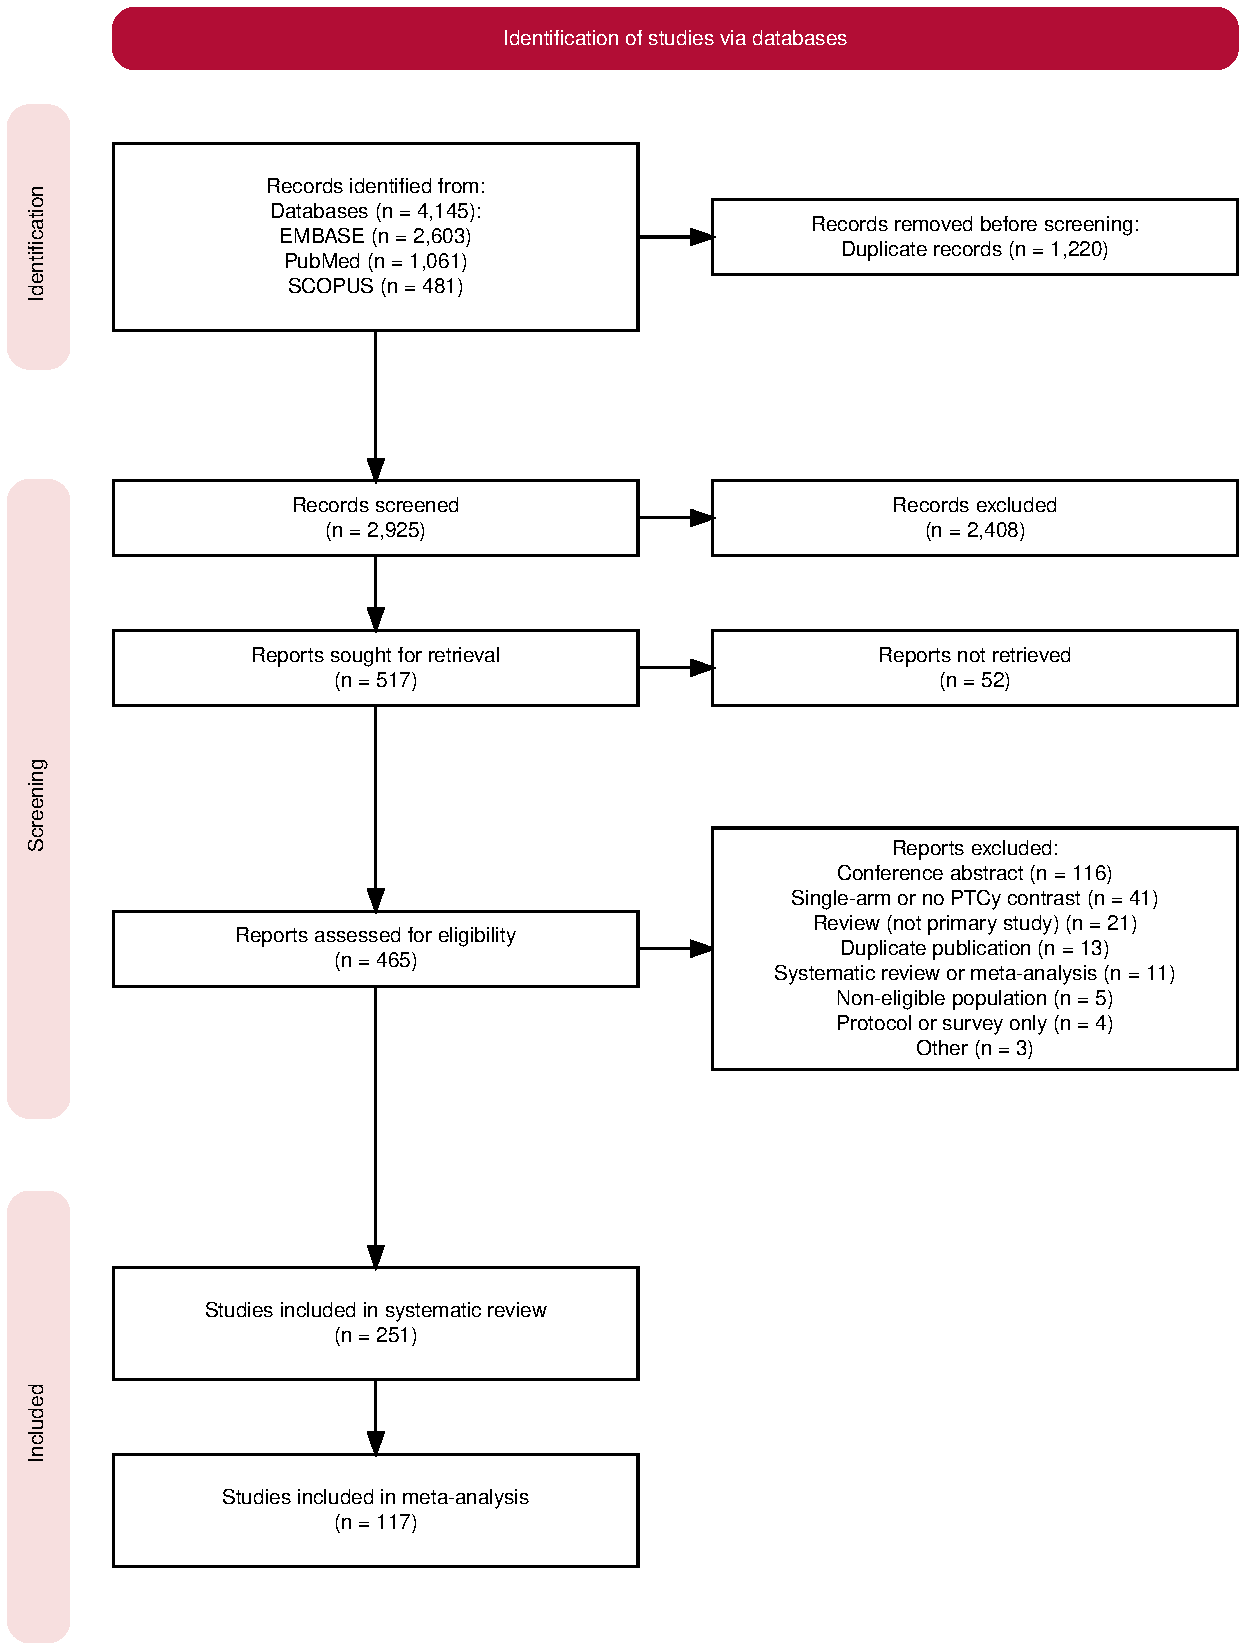
\includegraphics[keepaspectratio]{figures/Figure1_PRISMA_flow_diagram.pdf}}

}

\caption{\label{fig-prisma}\textbf{Study selection (PRISMA 2020 flow
diagram).} 4145 records were identified from databases (EMBASE 2603,
PubMed 1061, SCOPUS 481) and 1220 duplicates removed. 2925 records were
screened and 2408 excluded at title and abstract. 517 reports were
sought for retrieval; 52 were not retrieved or not in English. 465
full-text reports were assessed and 214 excluded
(\href{appendix-preview.html\#s2.-studies-excluded-at-full-text-screening-n214}{appendix
pp 6--14}). 251 studies were included in the systematic review; 117 with
extractable event counts were included in the meta-analysis (C1 83
studies; C2 42 studies; C3 13 studies).}

\end{figure}%

\newpage{}

\begin{figure}[tb]

\centering{

\pandocbounded{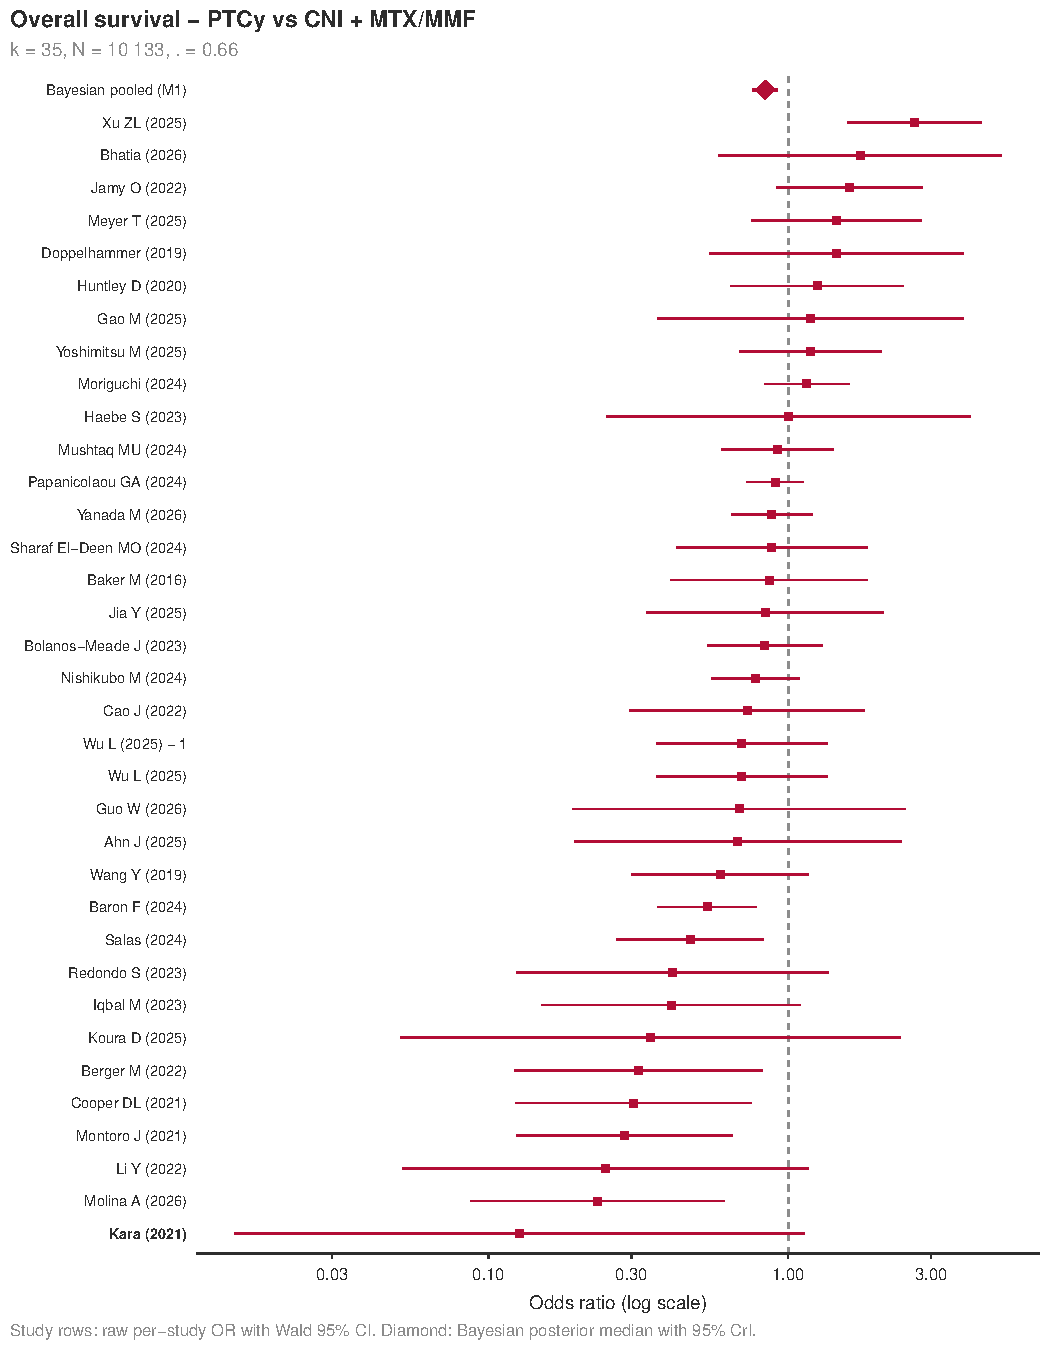
\includegraphics[keepaspectratio]{figures/Figure2_OS_forest_setB.pdf}}

}

\caption{\label{fig-os}\textbf{Forest plot --- overall survival,
comparison 1 (PTCy vs CNI + MTX/MMF).} Study rows are raw per-study odds
ratios with Wald 95\% CIs, computed from the extracted event counts; the
diamond is the pooled Bayesian random-effects posterior median with 95\%
credible interval (primary model M1). k = 35 after cohort
deduplication.}

\end{figure}%

\newpage{}

\begin{figure}[tb]

\begin{minipage}[t]{\linewidth}

\centering{

\pandocbounded{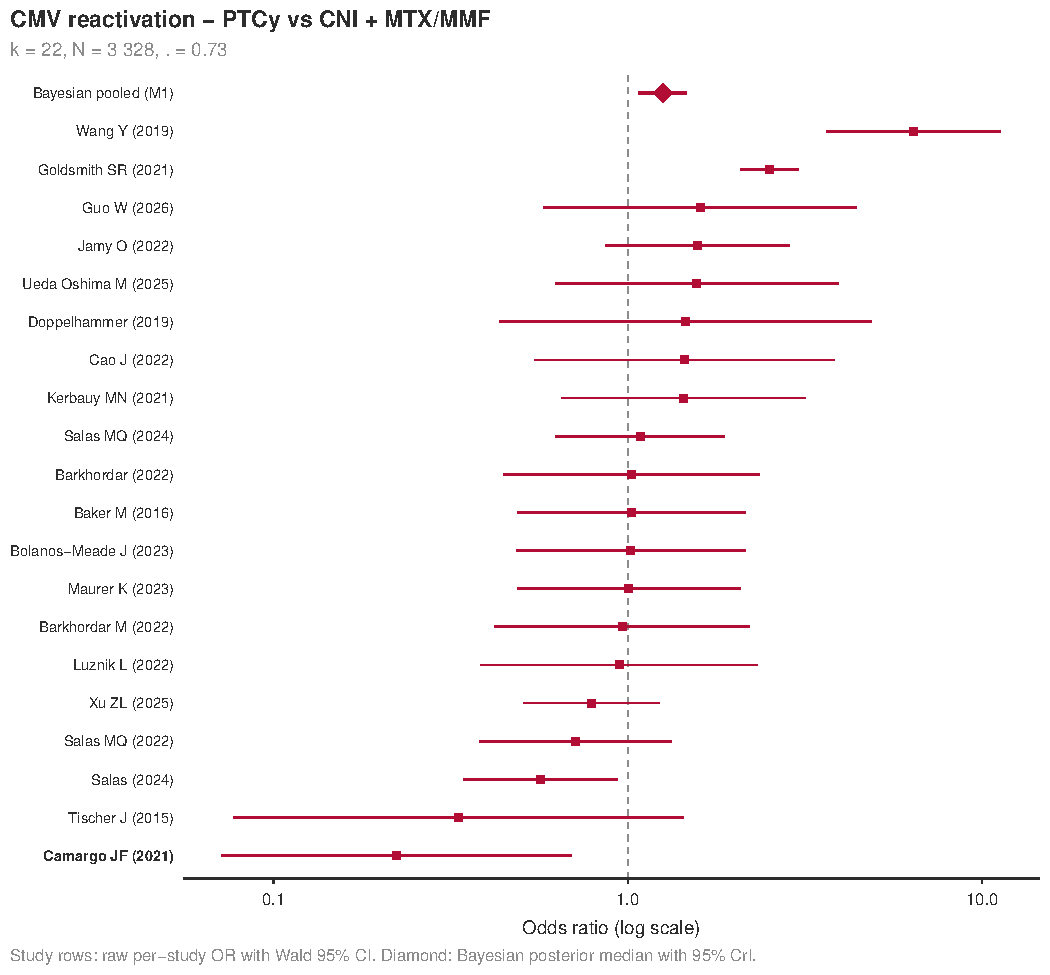
\includegraphics[keepaspectratio]{figures/Figure3a_CMV_C1_forest_setB.pdf}}

}

\subcaption{\label{fig-cmv-a}Comparison 1: PTCy vs CNI + MTX/MMF (k =
22, odds ratio 1·26 {[}1·07--1·47{]})}

\end{minipage}%
\newline
\begin{minipage}[t]{\linewidth}

\centering{

\pandocbounded{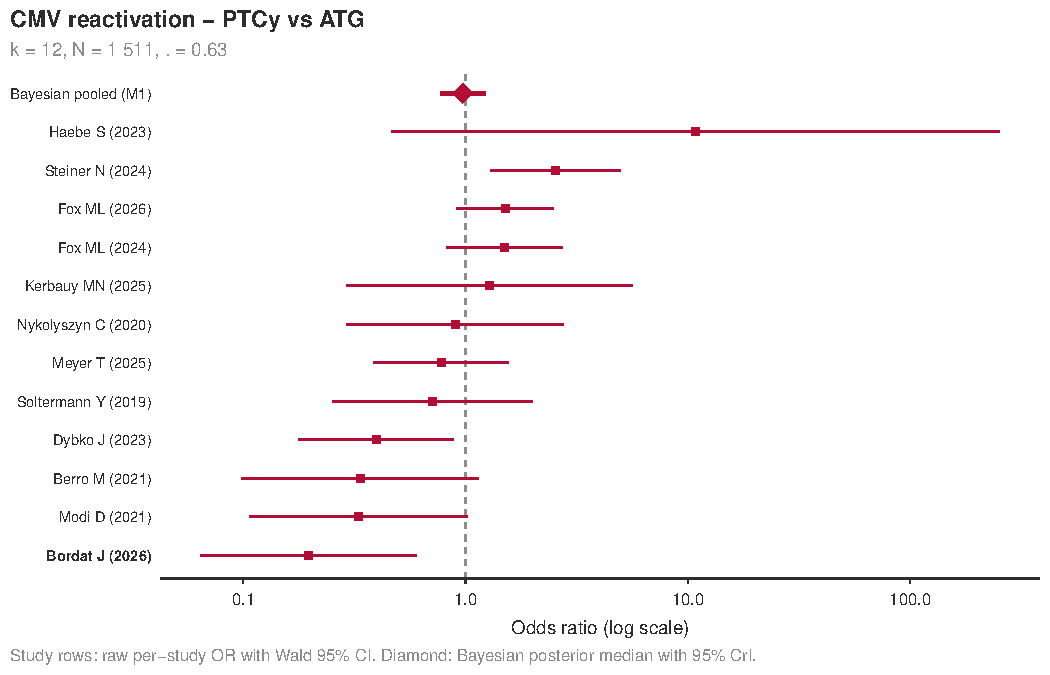
\includegraphics[keepaspectratio]{figures/Figure3b_CMV_C2_forest_setB.pdf}}

}

\subcaption{\label{fig-cmv-b}Comparison 2: PTCy vs ATG (k = 12, 0·97
{[}0·77--1·23{]})}

\end{minipage}%

\caption{\label{fig-cmv}\textbf{Forest plots --- CMV reactivation.}
Individual study odds ratios for any CMV reactivation, with the pooled
Bayesian posterior median and 95\% credible interval. CMV excess is seen
against CNI-based prophylaxis but not against ATG, consistent with a
T-cell depletion depth hierarchy.}

\end{figure}%

\newpage{}

\begin{figure}[tb]

\centering{

\pandocbounded{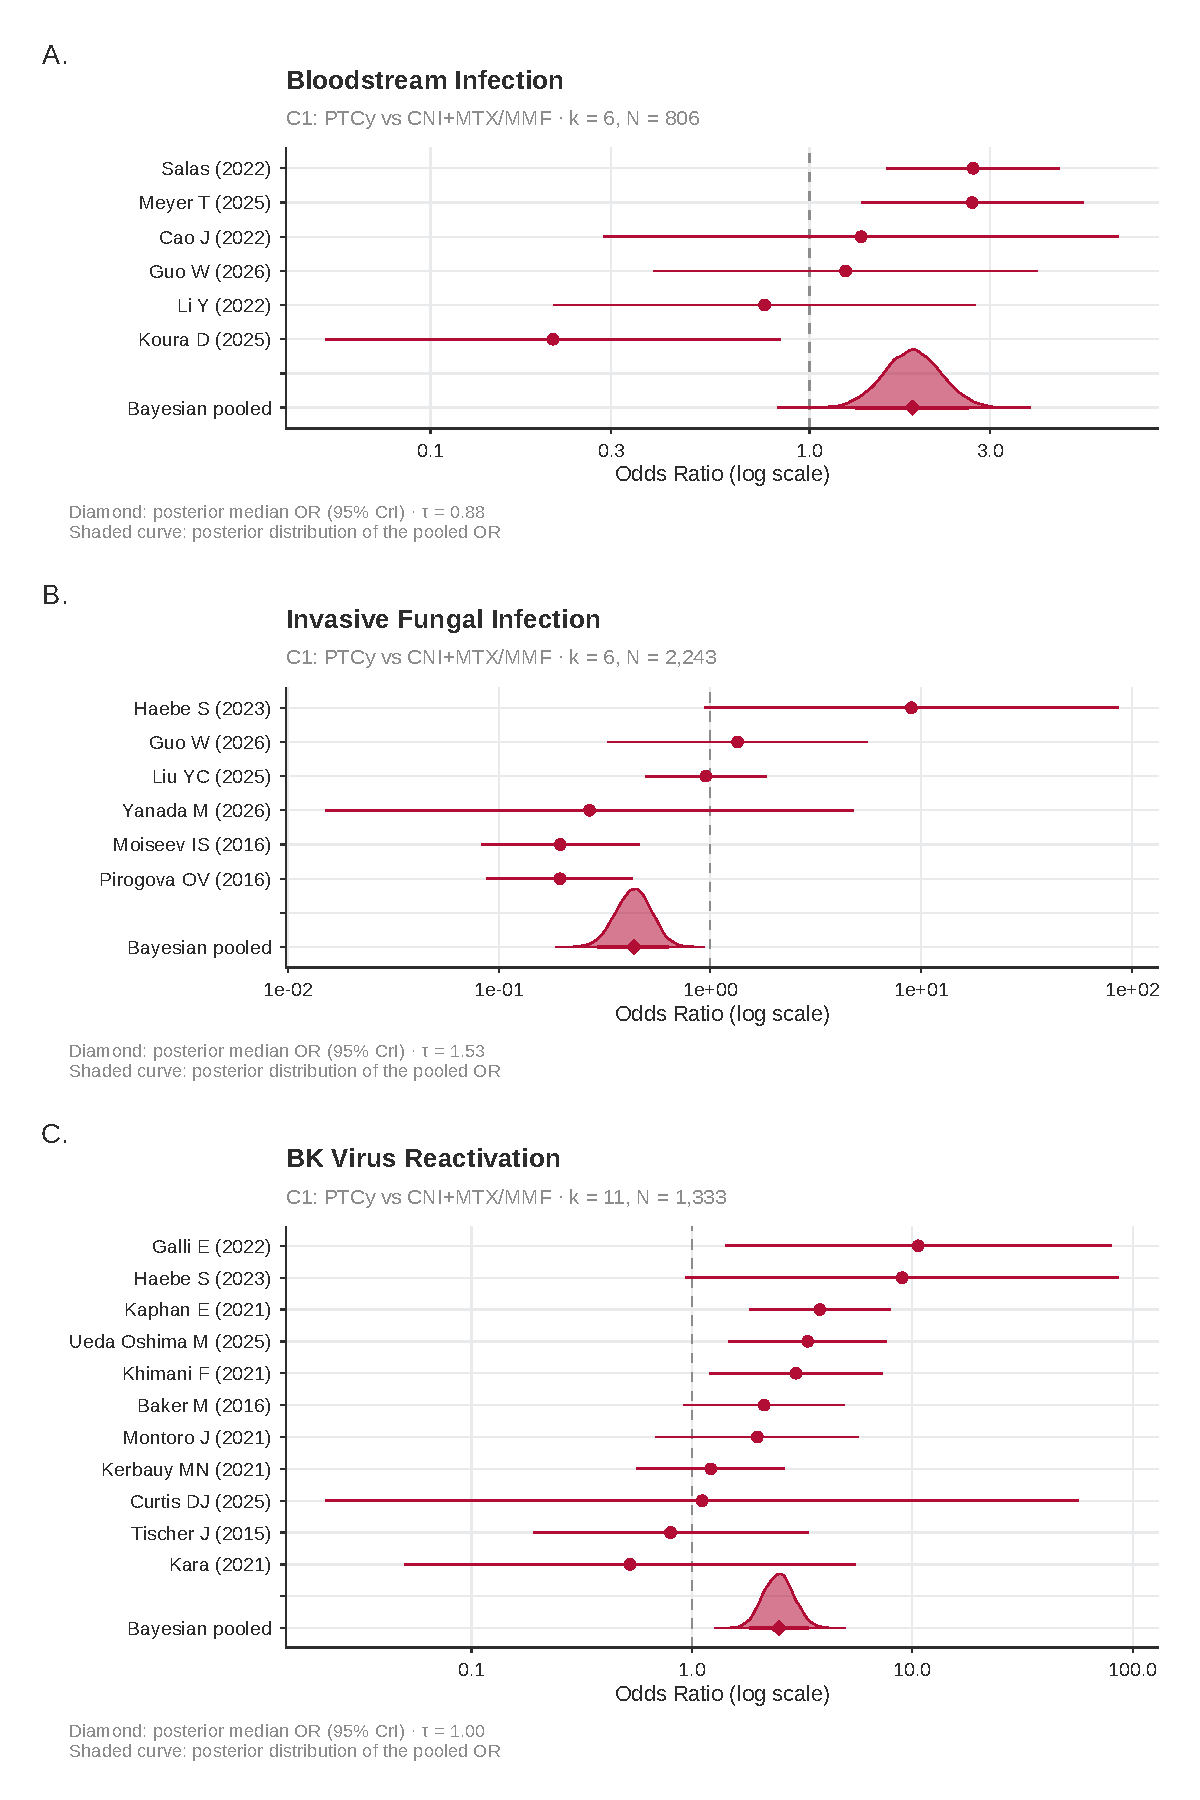
\includegraphics[keepaspectratio]{figures/Figure4_infections_forest.pdf}}

}

\caption{\label{fig-infections}\textbf{Forest plots --- bacterial,
fungal, and BK viral infection risk (comparison 1).} Individual study
odds ratios (raw per-study estimates) and pooled Bayesian random-effects
posterior median with 95\% credible interval (primary model M1), shown
with the posterior density above each pooled row. Panel A: bloodstream
infection, any pathogen (k = 6, odds ratio 1·87 {[}1·33--2·62{]}). Panel
B: invasive fungal infection, any (k = 6, 0·43 {[}0·29--0·63{]}; τ =
1·53). Panel C: BK virus reactivation (k = 11, 2·48 {[}1·82--3·38{]}),
the largest infection effect observed. All panels are comparison 1 (PTCy
versus CNI plus MTX or MMF); insufficient studies were available to fit
the corresponding comparison 2 models for BSI and IFI. None of these
three outcomes was affected by cohort deduplication.}

\end{figure}%




\end{document}
